\documentclass[10pt,a4paper]{article}
\usepackage[utf8]{inputenc} % para poder usar tildes en archivos UTF-8
\usepackage[spanish]{babel} % para que comandos como \today den el resultado en castellano
\usepackage{a4wide} % márgenes un poco más anchos que lo usual
\usepackage[conEntregas]{caratula}
\usepackage{ulem}
\usepackage{amsmath} 
\usepackage{amssymb}
\usepackage{fancybox}
\usepackage[usenames,dvipsnames]{color}
\usepackage{hyperref}
\usepackage{listings}
\usepackage{clrscode3e}
\usepackage{xcolor}
\usepackage{amsmath}
\usepackage{arydshln}
\usepackage{listings}

\hypersetup{
    colorlinks,
    citecolor=black,
    filecolor=black,
    linkcolor=black,
    urlcolor=black
}

\lstdefinestyle{customc}{
  belowcaptionskip=1\baselineskip,
  breaklines=true,
  frame=L,
  xleftmargin=\parindent,
  language=C,
  showstringspaces=false,
  basicstyle=\footnotesize\ttfamily,
  keywordstyle=\bfseries\color{green!40!black},
  commentstyle=\itshape\color{purple!40!black},
  identifierstyle=\color{blue},
  stringstyle=\color{orange},
}

\lstset{escapechar=@,style=customc}

\begin{document}

\titulo{Trabajo Práctico 2}
\subtitulo{[Primera entrega]}

\fecha{\today}

\materia{Bases de Datos}
\integrante{Fernandez, Esteban}{691/12}{esteban.pmf@gmail.com}
\integrante{Marta, Cristian G.}{079/12}{cristiangmarta@gmail.com}
\integrante{Wright, Carolina Rocío}{876/12}{wright.carolina@gmail.com}

\maketitle

\tableofcontents
\newpage

\section{Introducción}
Continuaremos el desarrollo del Sistema de seguimiento de casos policiales. Agregaremos una base de datos NoSQL basada en documentos (MongoDB) para guardar el historial de los casos. De esta forma podremos hacer consultas de manera más eficiente.

\section{Diseño NoSql}
Basándonos en el diseño entregado en el Trabajo Práctico 1, hemos creado el siguiente diagrama que refleja el contenido de los documentos que utilizaremos para realizar las consultas.

\begin{figure}[h]
	\centering
	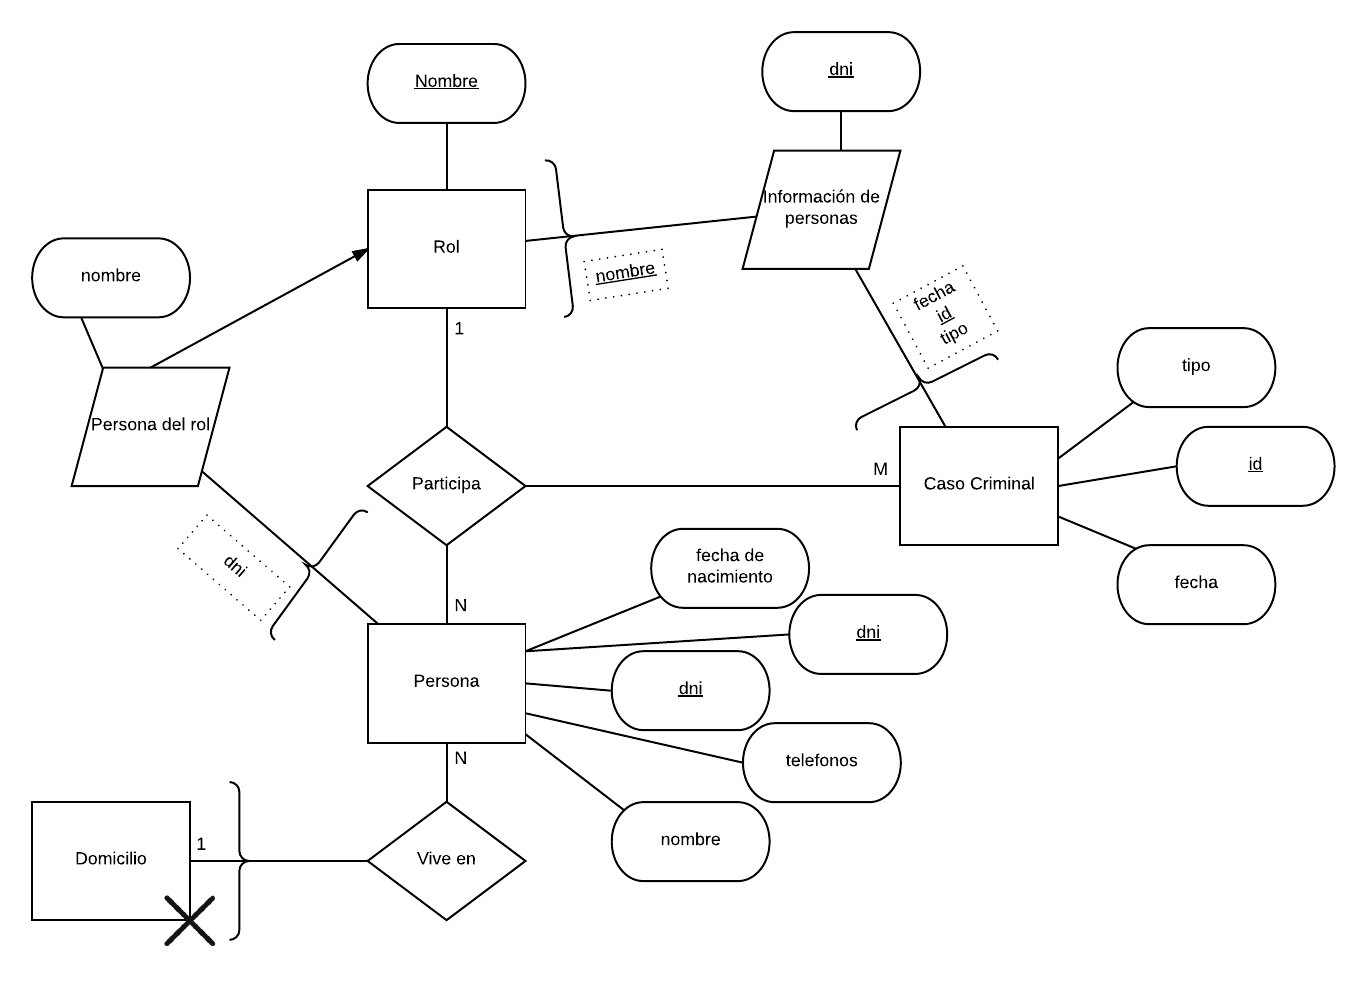
\includegraphics[width=\linewidth]{imagenes/DID.png}
\end{figure}

\subsection{JSON schemas}

\subsubsection{Información de personas}
\begin{lstlisting}
{"type":"object ",
	"properties":{
		"dni_persona": {"type":"integer"},
		"caso_y_rol": {"type":"array",
			"items":{"type":"object ",
				"properties":{
					"id":{"type":"integer"},
					"fecha_ingreso":{"type":"string", "format": "date"},
					"fecha":{"type":"string", "format": "date"},
					"lugar":{"type":"string"},
					"descripcion":{"type":"string"},
					"nombre_categoria":{"type":"string"},
					"estado":{"type":"string"},
					"nombre_rol": {"type":"string"}
				}
			}
		}
	}
}
\end{lstlisting}

Este documento se creó para resolver las siguientes consultas: personas involucradas como testigos en la mayor cantidad de casos y mayor número de crímenes cometido por alguna persona.
En ambas consultas buscamos información de las personas que participaron en casos criminales. Pudimos unificarlas en un mismo documento, agregando al mismo el rol en el caso (necesario para la primer consulta) y el nombre de la categoría del crímen (necesario para la segunda).

\subsubsection{Casos criminales}
\begin{lstlisting}
{"type":"object ",
	"properties":{
		"id": {"type":"integer"},
		"fecha_ingreso": {"type":"string", "format": "date"},
		"fecha": {"type":"string", "format": "date"},
		"lugar": {"type":"string"},
		"descripcion": {"type":"string"},
		"categoria": {"type":"string"},
		"evidencias": {"type":"array",
			"items":{"type":"object ",
				"properties":{
					"idEvidencia":{"type":"integer"}
				}
			}
		}
	}
}
\end{lstlisting}

Los casos criminales nos ayudaron a resolver: cantidad de crímenes por localidad y por año, y cantidad total de evidencias por caso.
Para ambas consultas necesitamos información de los casos. Para la primera la localidad y año, que son atributos de la entidad Caso criminal. Para la segunda, embebimos las evidencias en este documento que provienen de la relación Caso criminal - recolecta - Evidencia.

\subsection{Personas culpables}
\begin{lstlisting}
{"type":"object ",
	"properties":{
		"id_caso_criminal": {"type":"integer"},
		"personas_involucradas": {"type":"array",
			"items":{"type":"object ",
				"properties":{
					"dni_persona":{"type":"integer"}
				}
			}
		}
	}
}
\end{lstlisting}

Decidimos crear este documento para poder resolver la primera consulta: número promedio de crímenes cometidos por personas que ya han sido encontradas culpables de algún crimen.
De esta forma tenemos agrupadas las personas involucradas por caso criminal. Esto nos permitirá poder filtrar dentro de las personas involucradas a las culpables.

\subsection{Personas involucradas}
\begin{lstlisting}
{"type":"object ",
	"properties":{
		"id_caso_criminal": {"type":"integer"},
		"personas_involucradas": {"type":"array",
			"items":{"type":"object ",
				"properties":{
					"dni_persona":{"type":"integer"}
				}
			}
		}
	}
}
\end{lstlisting}
En este caso, el documento fue pensado para resolver: casos en los que se han visto involucradas el mayor número de personas. Agrupamos las personas involucradas en los casos criminales por caso. Tomando la cantidad de los involucrados ya podemos resolver la consulta.

\subsection{Categorías}
\begin{lstlisting}
{"type":"object ",
	"properties":{
		"nombre": {"type":"string"},
		"casos_criminales": {"type":"array",
			"items":{"type":"object ",
				"properties":{
					"id":{"type":"integer"},
					"lugar":{"type":"string"}
				}
			}
		}
	}
}
\end{lstlisting}
Este documento surge para poder resolver: las 10 ciudades con mayor número de crímenes. De esta forma tenemos agrupados los casos por categoría, en este caso nos concierne la categoría "Crimen" y de ella las ciudades. Por este motivo embebimos en Categoría los atributos id y lugar de Caso criminal.

\section{Parte 2 - Map Reduce}
A continuación se presentarán los algoritmos utilizados para resolver las consultas pedidas a partir de la utilización de Map-Reduce.

\subsection{Número promedio de crímenes cometidos por personas que ya han sido encontradas culpables de algún crimen}

\begin{lstlisting}
function map(){
	emit("acum", this.personas_culpables.length);
}

function reduce(acum_key, criminals){
	var amount_of_criminals = 0;
	var amount_of_criminal_cases = criminals.length; 
	
	for (var i = 0; i < amount_of_criminal_cases; i++) {
		amount_of_criminals += criminals[i];
	}

	return amount_of_criminals / amount_of_criminal_cases;
}

db.personasCulpables.mapReduce(map, reduce, {out: {inline: 1}})
\end{lstlisting}

En esta consulta, nos interesaba calcular el promedio de los crímenes. Es por ello que fuimos acumulando estos valores, todos juntos, para luego poder calcular el promedio sobre ellos.

\subsection{Personas involucradas como testigos en la mayor cantidad de casos}

\begin{lstlisting}
function map(){
	var witness_cases = this.caso_y_rol.filter( function(caso) {
		return caso.nombre_rol == "Testigo";});
	if (witness_cases.length > 0) 
		emit("acum", {dni: this.dni_persona, amount: witness_cases.length});
}


function reduce(acum, people) {

	var max_involved = [];
	var max_witnesses = 0;
	
	people.forEach( function(person) {
		if (person.amount > max_witnesses) {
			max_witnesses = person.amount;
			max_involved = [];
			max_involved.push(person.dni);
		}
		else if (person.amount == max_witnesses) {
			max_involved.push(person.dni);
		}
	})
	
	return {"result": max_involved};
}

db.informacionDePersonas.mapReduce(map, reduce, {out: {inline: 1}})
\end{lstlisting}


\subsection{Casos en los que se han visto involucradas el mayor número de personas}
\begin{lstlisting}
function map(){
	emit("acum", {id: this.id_caso_criminal, count: this.personas_involucradas.length});
}

function reduce(acum_key, cases) {
	var result_cases = [];
	var max_people = 0;
	
	cases.forEach( function(c) {
		if (c.count > max_people) {
			max_people = c.count;
			result_cases = [];
			result_cases.push(c.id);
		}
		else if (c.count == max_people) {
			result_cases.push(c.id);
		}
	});
	return {"result": result_cases};
}

db.personasInvolucradas.mapReduce(map, reduce, {out: {inline: 1}})
\end{lstlisting}

Como buscamos de entre todos los casos, los que hayan tenido involucrados mayor cantidad de personas, nos pareció conveniente acumular estos valores y luego filtar para quedarnos con los que efectivamente cumplen lo buscado.
El map-reduce se hace sobre la colección de personas involucradas que contiene para cada caso, una lista de las personas involucradas.

\subsection{Cantidad de crímenes por localidad y por año}

\begin{lstlisting}
function map(){
	var year = new Date(Date.parse(this.fecha)).getFullYear();
	emit(this.lugar + year, 1);
}

function reduce(cityAndYear, count){
	return count.length;
}

db.casosCriminales.mapReduce(map, reduce, {out: {inline: 1}})
\end{lstlisting}

En este caso, la función map agrega por cada caso que sucede en un lugar-año un elemento a la lista relacionada con ese lugar-año. Luego en la función reduce solo resta tomar el tamaño de esa lista para obtener la cantidad de crímenes asociados a esa localidad y año (pues por cada caso criminal se agrego un elemento a la lista).

\subsection{Mayor número de crímenes cometido por alguna persona}
\begin{lstlisting}

function map(){
	var crimes = this.caso_y_rol.filter( function(caso) {
		return caso.nombre_categoria == "Crimen";
	})
	if (crimes.length > 0) 
		emit("acum", crimes.length);
	
}

function reduce(acum, crimes_quantities) {
	return Math.max.apply(crimes_quantities);
}

db.informacionDePersonas.mapReduce(map, reduce, {out: {inline: 1}})
\end{lstlisting}


\subsection{Cantidad total de evidencias por caso}

\begin{lstlisting}
function map(){
	emit(this.id, this.evidencias);
}

function reduce(case_id, evidences){
	return evidences.length;
}

db.casosCriminales.mapReduce(map, reduce, {out: {inline: 1}})
\end{lstlisting}

En esta consulta agrupamos por cada caso criminal, sus evidencias.

\subsection{Las 10 ciudades con mayor número de crímenes}
\begin{lstlisting}

function map(){
	if (this.nombre == "Crimen") {
		emit(this.nombre, this.casos_criminales);
	}	
}

function reduce(crime, cases){
    var groupedByCity = groupByCity(cases);
    
    groupedByCity.sort( function(a, b) {
        return ((a["count"] >= b["count"]) ? 1 : -1);
    });
    
    return groupedByCity.slice(0, 10).map( function(elem) {
    	return elem.city;
    });
}

db.system.js.save(function groupByCity(cases) {
	var groups = {};

	for(var i = 0; i < cases.length; i++) {
		var item = cases[i];

		if(!groups[item.lugar]) {
		    groups[item.lugar] = 0;
		}

		groups[item.lugar] = groups[item.lugar] + 1;
	}
	
	var result_cases;
	for (var group in groups) {
  		result_cases.push({city: group, count: groups[group]});
	}
	return groups;
})
\end{lstlisting}
\subsection{Conclusión}
Nuestra conclusión es que, conociendo las consultas más frecuentes, podemos modelar nuestra base de datos para poder recuperar la información asociada a estas consultas de una manera mucho más rápida: utilizando el modelo NoSQL. Esto nos permite evitar mantener bases de datos Relacionales SQL que requieren operaciones costosas de recuperación y joineo de tablas para consultar la información que sabemos de ante mano será consultada. Es por esto que el modelo NOSQL supera en este punto a las bases NoSQL: los documentos ya almacenan lo que necesitamos precisamente. Luego podemos consultar directamente por Key o bien relacionar las diferentes entradas de los documentos utilizando MapReduce para transformar y combinar dichas diferentes entradas de los documentos.

\end{document}